\begin{figure*}[t]
\centering
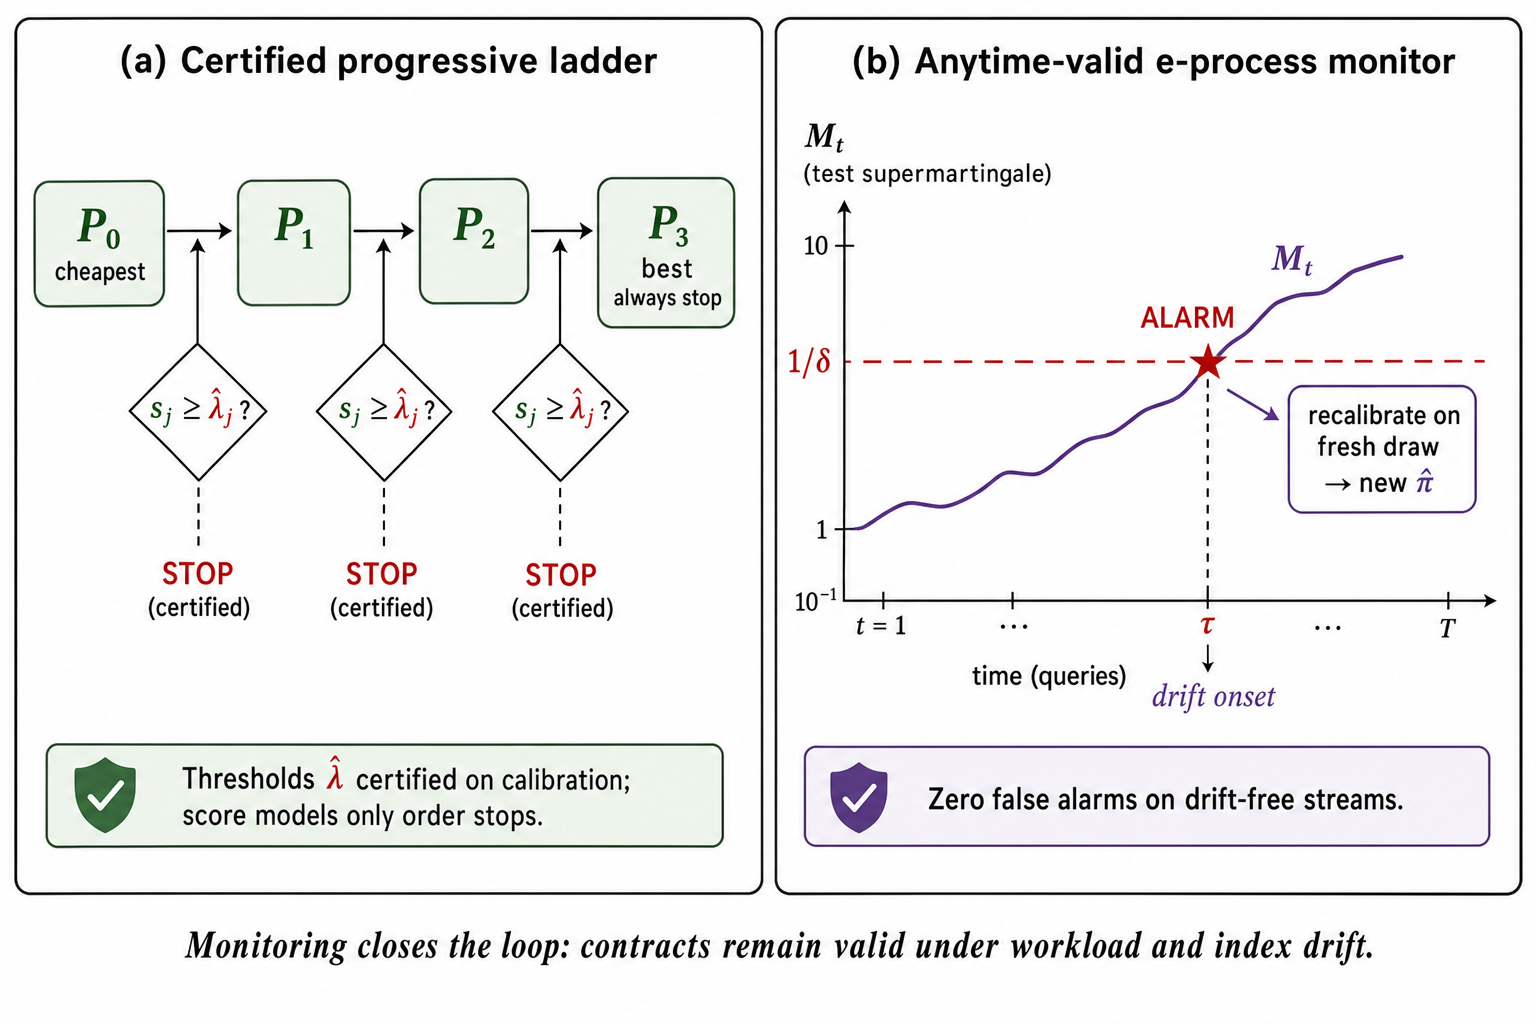
\includegraphics[width=0.95\textwidth]{figures/fig_runtime_imagegen.png}
\caption{Progressive execution and online monitoring.
(a)~A certified escalation ladder stops at the first rung whose
sufficiency score clears the calibration-certified threshold
$\hat\lambda_j$; scores only order stops, thresholds carry the
guarantee (Theorem~\ref{thm:validity}).
(b)~The anytime-valid e-process $M_t$ alarms when it crosses
$1/\delta$, triggering recalibration; under the contract it has
false-alarm probability $\le\delta$ (Proposition~\ref{prop:eprocess}).}
\Description{A progressive execution ladder escalates through stronger
plans, while an anytime-valid monitor observes audited contract losses
and triggers recalibration after a detected shift.}
\label{fig:runtime}
\end{figure*}
